\documentclass{standalone}
\usepackage{tikz}
\usetikzlibrary{patterns, positioning}
\usepackage[sfdefault]{ClearSans} %% option 'sfdefault' activates Clear Sans as the default text font
\usepackage[T1]{fontenc}

\begin{document}
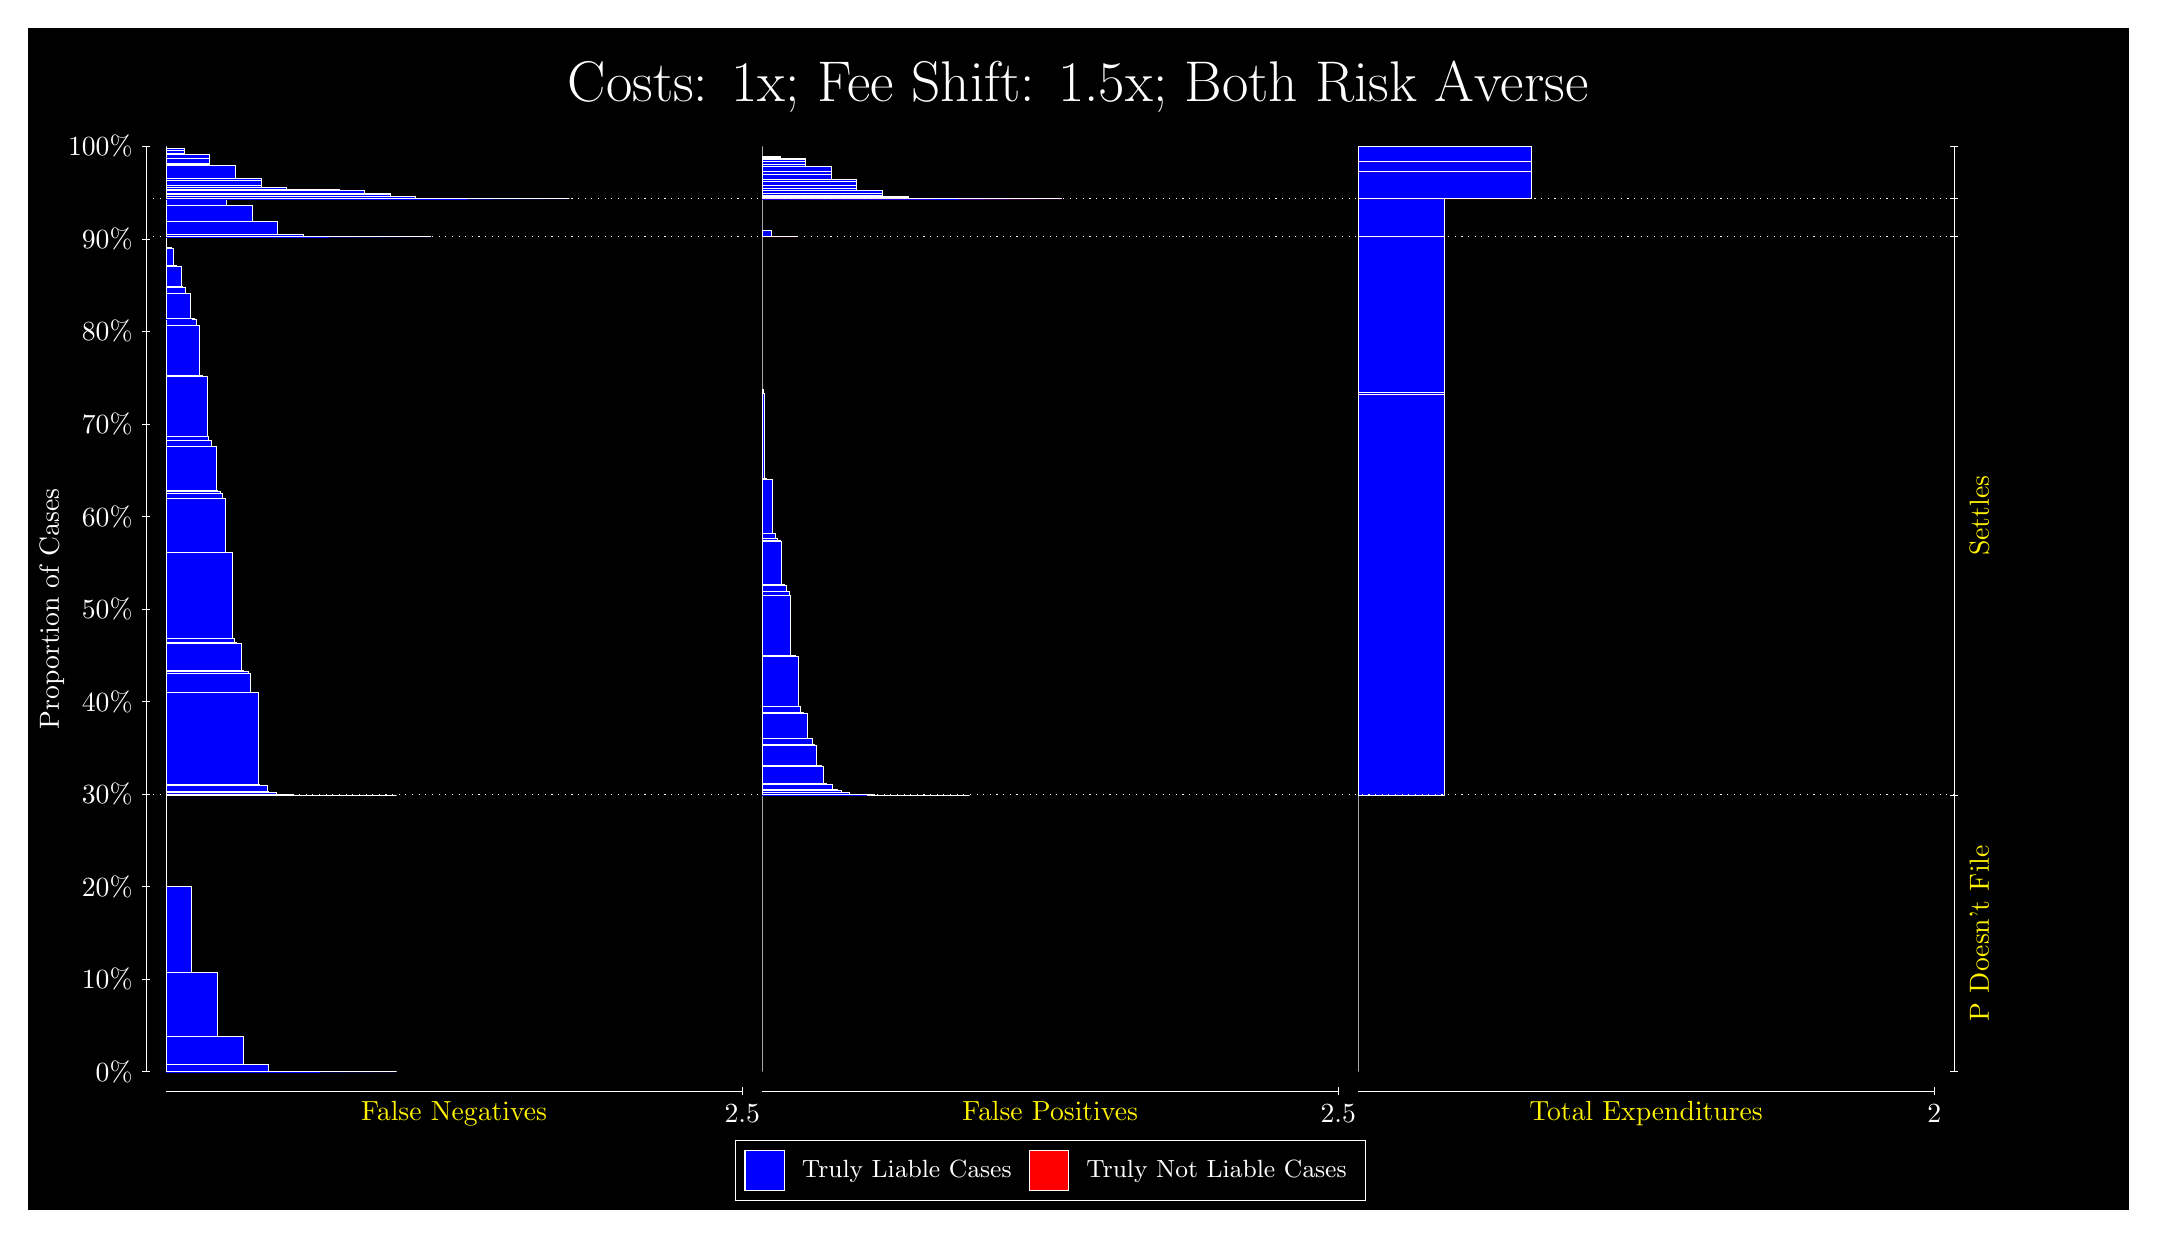
\begin{tikzpicture}
\draw[fill=black] (0,0) rectangle (26.667,15);
\draw[text=white] (0,13.5) rectangle (26.667,15) node[midway] {\huge Costs: 1x; Fee Shift: 1.5x; Both Risk Averse};
\draw[white, very thin] (1.5,1.75) -- (1.5,13.5);
\node[rotate=90, text=white, anchor=center] at (0.3, 7.625) {Proportion of Cases};
\draw[white, very thin] (1.45,1.75) -- (1.55,1.75);
\node[text=white, anchor=east] at (1.45, 1.75) {0\%};
\draw[white, very thin] (1.45,2.925) -- (1.55,2.925);
\node[text=white, anchor=east] at (1.45, 2.925) {10\%};
\draw[white, very thin] (1.45,4.1) -- (1.55,4.1);
\node[text=white, anchor=east] at (1.45, 4.1) {20\%};
\draw[white, very thin] (1.45,5.275) -- (1.55,5.275);
\node[text=white, anchor=east] at (1.45, 5.275) {30\%};
\draw[white, very thin] (1.45,6.45) -- (1.55,6.45);
\node[text=white, anchor=east] at (1.45, 6.45) {40\%};
\draw[white, very thin] (1.45,7.625) -- (1.55,7.625);
\node[text=white, anchor=east] at (1.45, 7.625) {50\%};
\draw[white, very thin] (1.45,8.8) -- (1.55,8.8);
\node[text=white, anchor=east] at (1.45, 8.8) {60\%};
\draw[white, very thin] (1.45,9.975) -- (1.55,9.975);
\node[text=white, anchor=east] at (1.45, 9.975) {70\%};
\draw[white, very thin] (1.45,11.15) -- (1.55,11.15);
\node[text=white, anchor=east] at (1.45, 11.15) {80\%};
\draw[white, very thin] (1.45,12.325) -- (1.55,12.325);
\node[text=white, anchor=east] at (1.45, 12.325) {90\%};
\draw[white, very thin] (1.45,13.5) -- (1.55,13.5);
\node[text=white, anchor=east] at (1.45, 13.5) {100\%};

\draw[white, very thin] (24.457,1.75) -- (24.457,13.5);
\draw[white, very thin] (24.407,1.75) -- (24.507,1.75);
\node[anchor=west] at (24.407, 1.75) {};
\draw[white, very thin] (24.407,5.264) -- (24.507,5.264);
\node[anchor=west] at (24.407, 5.264) {};
\draw[white, very thin] (24.407,12.352) -- (24.507,12.352);
\node[anchor=west] at (24.407, 12.352) {};
\draw[white, very thin] (24.407,12.835) -- (24.507,12.835);
\node[anchor=west] at (24.407, 12.835) {};
\draw[white, very thin] (24.407,13.5) -- (24.507,13.5);
\node[anchor=west] at (24.407, 13.5) {};

\draw[white, very thin, fill=blue] (1.75,1.75) rectangle (4.6775,1.75);
\draw[white, very thin, fill=blue] (1.75,1.75) rectangle (4.3523,1.75);
\draw[white, very thin, fill=blue] (1.75,1.75) rectangle (4.027,1.75);
\draw[white, very thin, fill=blue] (1.75,1.75) rectangle (3.7017,1.7503);
\draw[white, very thin, fill=blue] (1.75,1.7503) rectangle (3.3764,1.7576);
\draw[white, very thin, fill=blue] (1.75,1.7576) rectangle (3.0511,1.8361);
\draw[white, very thin, fill=blue] (1.75,1.8361) rectangle (2.7258,2.1984);
\draw[white, very thin, fill=blue] (1.75,2.1984) rectangle (2.4006,3.0086);
\draw[white, very thin, fill=blue] (1.75,3.0086) rectangle (2.0753,4.0995);
\draw[white, very thin, fill=red] (1.75,4.0995) rectangle (1.75,4.0995);
\draw[white, very thin, fill=blue] (1.75,4.0995) rectangle (1.75,5.264);
\draw[white, very thin, fill=blue] (1.75,5.264) rectangle (4.6775,5.264);
\draw[white, very thin, fill=blue] (1.75,5.264) rectangle (4.5312,5.264);
\draw[white, very thin, fill=blue] (1.75,5.264) rectangle (4.3848,5.264);
\draw[white, very thin, fill=blue] (1.75,5.264) rectangle (4.3523,5.264);
\draw[white, very thin, fill=blue] (1.75,5.264) rectangle (4.2384,5.264);
\draw[white, very thin, fill=blue] (1.75,5.264) rectangle (4.2059,5.264);
\draw[white, very thin, fill=blue] (1.75,5.264) rectangle (4.092,5.264);
\draw[white, very thin, fill=blue] (1.75,5.264) rectangle (4.0595,5.264);
\draw[white, very thin, fill=blue] (1.75,5.264) rectangle (4.027,5.264);
\draw[white, very thin, fill=blue] (1.75,5.264) rectangle (3.9457,5.264);
\draw[white, very thin, fill=blue] (1.75,5.264) rectangle (3.9131,5.264);
\draw[white, very thin, fill=blue] (1.75,5.264) rectangle (3.8806,5.264);
\draw[white, very thin, fill=blue] (1.75,5.264) rectangle (3.7993,5.264);
\draw[white, very thin, fill=blue] (1.75,5.264) rectangle (3.7668,5.264);
\draw[white, very thin, fill=blue] (1.75,5.264) rectangle (3.7342,5.264);
\draw[white, very thin, fill=blue] (1.75,5.264) rectangle (3.7017,5.264);
\draw[white, very thin, fill=blue] (1.75,5.264) rectangle (3.6529,5.264);
\draw[white, very thin, fill=blue] (1.75,5.264) rectangle (3.6204,5.264);
\draw[white, very thin, fill=blue] (1.75,5.264) rectangle (3.5878,5.264);
\draw[white, very thin, fill=blue] (1.75,5.264) rectangle (3.5553,5.264);
\draw[white, very thin, fill=blue] (1.75,5.264) rectangle (3.5065,5.264);
\draw[white, very thin, fill=blue] (1.75,5.264) rectangle (3.474,5.2645);
\draw[white, very thin, fill=blue] (1.75,5.2645) rectangle (3.4415,5.2645);
\draw[white, very thin, fill=blue] (1.75,5.2645) rectangle (3.4089,5.2645);
\draw[white, very thin, fill=blue] (1.75,5.2645) rectangle (3.3764,5.2647);
\draw[white, very thin, fill=blue] (1.75,5.2647) rectangle (3.3602,5.2752);
\draw[white, very thin, fill=blue] (1.75,5.2752) rectangle (3.3276,5.2752);
\draw[white, very thin, fill=blue] (1.75,5.2752) rectangle (3.2951,5.2752);
\draw[white, very thin, fill=blue] (1.75,5.2752) rectangle (3.2626,5.2757);
\draw[white, very thin, fill=blue] (1.75,5.2757) rectangle (3.23,5.2759);
\draw[white, very thin, fill=blue] (1.75,5.2759) rectangle (3.1812,5.2759);
\draw[white, very thin, fill=blue] (1.75,5.2759) rectangle (3.1487,5.3004);
\draw[white, very thin, fill=blue] (1.75,5.3004) rectangle (3.1162,5.3011);
\draw[white, very thin, fill=blue] (1.75,5.3011) rectangle (3.0837,5.3015);
\draw[white, very thin, fill=blue] (1.75,5.3015) rectangle (3.0511,5.3044);
\draw[white, very thin, fill=blue] (1.75,5.3044) rectangle (3.0349,5.388);
\draw[white, very thin, fill=blue] (1.75,5.388) rectangle (3.0023,5.3881);
\draw[white, very thin, fill=blue] (1.75,5.3881) rectangle (2.9698,5.3888);
\draw[white, very thin, fill=blue] (1.75,5.3888) rectangle (2.9373,5.3988);
\draw[white, very thin, fill=blue] (1.75,5.3988) rectangle (2.921,6.5628);
\draw[white, very thin, fill=blue] (1.75,6.5628) rectangle (2.9048,6.5663);
\draw[white, very thin, fill=blue] (1.75,6.5663) rectangle (2.856,6.5664);
\draw[white, very thin, fill=blue] (1.75,6.5664) rectangle (2.8234,6.8137);
\draw[white, very thin, fill=blue] (1.75,6.8137) rectangle (2.7909,6.8283);
\draw[white, very thin, fill=blue] (1.75,6.8283) rectangle (2.7584,6.8355);
\draw[white, very thin, fill=blue] (1.75,6.8355) rectangle (2.7258,6.8492);
\draw[white, very thin, fill=blue] (1.75,6.8492) rectangle (2.7096,7.1892);
\draw[white, very thin, fill=blue] (1.75,7.1892) rectangle (2.6771,7.1907);
\draw[white, very thin, fill=blue] (1.75,7.1907) rectangle (2.6445,7.2067);
\draw[white, very thin, fill=blue] (1.75,7.2067) rectangle (2.612,7.2545);
\draw[white, very thin, fill=blue] (1.75,7.2545) rectangle (2.5957,8.3382);
\draw[white, very thin, fill=blue] (1.75,8.3382) rectangle (2.5795,8.3468);
\draw[white, very thin, fill=blue] (1.75,8.3468) rectangle (2.5307,8.3485);
\draw[white, very thin, fill=blue] (1.75,8.3485) rectangle (2.4982,9.0277);
\draw[white, very thin, fill=blue] (1.75,9.0277) rectangle (2.4656,9.0966);
\draw[white, very thin, fill=blue] (1.75,9.0966) rectangle (2.4331,9.1148);
\draw[white, very thin, fill=blue] (1.75,9.1148) rectangle (2.4006,9.1268);
\draw[white, very thin, fill=blue] (1.75,9.1268) rectangle (2.3843,9.6843);
\draw[white, very thin, fill=blue] (1.75,9.6843) rectangle (2.3518,9.691);
\draw[white, very thin, fill=blue] (1.75,9.691) rectangle (2.3192,9.764);
\draw[white, very thin, fill=blue] (1.75,9.764) rectangle (2.2867,9.8194);
\draw[white, very thin, fill=blue] (1.75,9.8194) rectangle (2.2705,10.575);
\draw[white, very thin, fill=blue] (1.75,10.575) rectangle (2.2542,10.579);
\draw[white, very thin, fill=blue] (1.75,10.579) rectangle (2.2054,10.586);
\draw[white, very thin, fill=blue] (1.75,10.586) rectangle (2.1729,11.225);
\draw[white, very thin, fill=blue] (1.75,11.225) rectangle (2.1403,11.303);
\draw[white, very thin, fill=blue] (1.75,11.303) rectangle (2.1078,11.31);
\draw[white, very thin, fill=blue] (1.75,11.31) rectangle (2.0753,11.312);
\draw[white, very thin, fill=blue] (1.75,11.312) rectangle (2.059,11.629);
\draw[white, very thin, fill=blue] (1.75,11.629) rectangle (2.0265,11.635);
\draw[white, very thin, fill=blue] (1.75,11.635) rectangle (1.994,11.713);
\draw[white, very thin, fill=blue] (1.75,11.713) rectangle (1.9614,11.727);
\draw[white, very thin, fill=blue] (1.75,11.727) rectangle (1.9452,11.978);
\draw[white, very thin, fill=blue] (1.75,11.978) rectangle (1.9289,11.978);
\draw[white, very thin, fill=blue] (1.75,11.978) rectangle (1.8801,11.985);
\draw[white, very thin, fill=blue] (1.75,11.985) rectangle (1.8476,12.199);
\draw[white, very thin, fill=blue] (1.75,12.199) rectangle (1.8151,12.22);
\draw[white, very thin, fill=blue] (1.75,12.22) rectangle (1.7825,12.22);
\draw[white, very thin, fill=red] (1.75,12.22) rectangle (1.75,12.22);
\draw[white, very thin, fill=blue] (1.75,12.22) rectangle (1.75,12.352);
\draw[white, very thin, fill=blue] (1.75,12.352) rectangle (5.1167,12.352);
\draw[white, very thin, fill=blue] (1.75,12.352) rectangle (4.7914,12.352);
\draw[white, very thin, fill=blue] (1.75,12.352) rectangle (4.4661,12.352);
\draw[white, very thin, fill=blue] (1.75,12.352) rectangle (4.1408,12.352);
\draw[white, very thin, fill=blue] (1.75,12.352) rectangle (3.8155,12.354);
\draw[white, very thin, fill=blue] (1.75,12.354) rectangle (3.4903,12.387);
\draw[white, very thin, fill=blue] (1.75,12.387) rectangle (3.165,12.553);
\draw[white, very thin, fill=blue] (1.75,12.553) rectangle (2.8397,12.755);
\draw[white, very thin, fill=blue] (1.75,12.755) rectangle (2.5144,12.825);
\draw[white, very thin, fill=blue] (1.75,12.825) rectangle (2.1891,12.835);
\draw[white, very thin, fill=red] (1.75,12.835) rectangle (1.75,12.835);
\draw[white, very thin, fill=blue] (1.75,12.835) rectangle (6.8732,12.835);
\draw[white, very thin, fill=blue] (1.75,12.835) rectangle (6.5479,12.835);
\draw[white, very thin, fill=blue] (1.75,12.835) rectangle (6.2226,12.835);
\draw[white, very thin, fill=blue] (1.75,12.835) rectangle (5.8974,12.835);
\draw[white, very thin, fill=blue] (1.75,12.835) rectangle (5.8974,12.835);
\draw[white, very thin, fill=blue] (1.75,12.835) rectangle (5.5721,12.836);
\draw[white, very thin, fill=blue] (1.75,12.836) rectangle (5.5721,12.836);
\draw[white, very thin, fill=blue] (1.75,12.836) rectangle (5.2468,12.839);
\draw[white, very thin, fill=blue] (1.75,12.839) rectangle (5.2305,12.839);
\draw[white, very thin, fill=blue] (1.75,12.839) rectangle (4.9215,12.844);
\draw[white, very thin, fill=blue] (1.75,12.844) rectangle (4.9215,12.86);
\draw[white, very thin, fill=blue] (1.75,12.86) rectangle (4.9052,12.86);
\draw[white, very thin, fill=blue] (1.75,12.86) rectangle (4.5962,12.867);
\draw[white, very thin, fill=blue] (1.75,12.867) rectangle (4.5962,12.896);
\draw[white, very thin, fill=blue] (1.75,12.896) rectangle (4.5962,12.908);
\draw[white, very thin, fill=blue] (1.75,12.908) rectangle (4.58,12.908);
\draw[white, very thin, fill=blue] (1.75,12.908) rectangle (4.58,12.908);
\draw[white, very thin, fill=blue] (1.75,12.908) rectangle (4.2709,12.939);
\draw[white, very thin, fill=blue] (1.75,12.939) rectangle (4.2709,12.944);
\draw[white, very thin, fill=blue] (1.75,12.944) rectangle (4.2547,12.944);
\draw[white, very thin, fill=blue] (1.75,12.944) rectangle (4.2547,12.944);
\draw[white, very thin, fill=blue] (1.75,12.944) rectangle (3.9457,12.954);
\draw[white, very thin, fill=blue] (1.75,12.954) rectangle (3.9294,12.954);
\draw[white, very thin, fill=blue] (1.75,12.954) rectangle (3.6204,12.955);
\draw[white, very thin, fill=blue] (1.75,12.955) rectangle (3.6041,12.957);
\draw[white, very thin, fill=blue] (1.75,12.957) rectangle (3.2951,12.957);
\draw[white, very thin, fill=blue] (1.75,12.957) rectangle (3.2788,12.96);
\draw[white, very thin, fill=blue] (1.75,12.96) rectangle (3.2788,12.983);
\draw[white, very thin, fill=blue] (1.75,12.983) rectangle (2.9698,12.983);
\draw[white, very thin, fill=blue] (1.75,12.983) rectangle (2.9535,12.983);
\draw[white, very thin, fill=blue] (1.75,12.983) rectangle (2.9535,13.004);
\draw[white, very thin, fill=blue] (1.75,13.004) rectangle (2.9535,13.063);
\draw[white, very thin, fill=blue] (1.75,13.063) rectangle (2.9535,13.089);
\draw[white, very thin, fill=blue] (1.75,13.089) rectangle (2.6445,13.089);
\draw[white, very thin, fill=blue] (1.75,13.089) rectangle (2.6283,13.092);
\draw[white, very thin, fill=blue] (1.75,13.092) rectangle (2.6283,13.256);
\draw[white, very thin, fill=blue] (1.75,13.256) rectangle (2.303,13.268);
\draw[white, very thin, fill=blue] (1.75,13.268) rectangle (2.303,13.287);
\draw[white, very thin, fill=blue] (1.75,13.287) rectangle (2.303,13.342);
\draw[white, very thin, fill=blue] (1.75,13.342) rectangle (2.303,13.398);
\draw[white, very thin, fill=blue] (1.75,13.398) rectangle (1.9777,13.417);
\draw[white, very thin, fill=blue] (1.75,13.417) rectangle (1.9777,13.452);
\draw[white, very thin, fill=blue] (1.75,13.452) rectangle (1.9777,13.472);
\draw[white, very thin, fill=red] (1.75,13.472) rectangle (1.75,13.472);
\draw[white, very thin, fill=blue] (1.75,13.472) rectangle (1.75,13.5);
\draw[white, very thin, fill=red] (9.3189,1.75) rectangle (9.3189,1.75);
\draw[white, very thin, fill=blue] (9.3189,1.75) rectangle (9.3189,5.264);
\draw[white, very thin, fill=red] (9.3189,5.264) rectangle (11.954,5.264);
\draw[white, very thin, fill=blue] (9.3189,5.264) rectangle (11.954,5.264);
\draw[white, very thin, fill=blue] (9.3189,5.264) rectangle (11.628,5.264);
\draw[white, very thin, fill=red] (9.3189,5.264) rectangle (11.515,5.264);
\draw[white, very thin, fill=blue] (9.3189,5.264) rectangle (11.515,5.264);
\draw[white, very thin, fill=red] (9.3189,5.264) rectangle (11.368,5.264);
\draw[white, very thin, fill=blue] (9.3189,5.264) rectangle (11.368,5.264);
\draw[white, very thin, fill=blue] (9.3189,5.264) rectangle (11.303,5.264);
\draw[white, very thin, fill=red] (9.3189,5.264) rectangle (11.222,5.264);
\draw[white, very thin, fill=blue] (9.3189,5.264) rectangle (11.222,5.264);
\draw[white, very thin, fill=blue] (9.3189,5.264) rectangle (11.189,5.264);
\draw[white, very thin, fill=red] (9.3189,5.264) rectangle (11.075,5.264);
\draw[white, very thin, fill=blue] (9.3189,5.264) rectangle (11.075,5.264);
\draw[white, very thin, fill=blue] (9.3189,5.264) rectangle (11.043,5.264);
\draw[white, very thin, fill=blue] (9.3189,5.264) rectangle (10.978,5.264);
\draw[white, very thin, fill=red] (9.3189,5.264) rectangle (10.929,5.264);
\draw[white, very thin, fill=blue] (9.3189,5.264) rectangle (10.929,5.264);
\draw[white, very thin, fill=blue] (9.3189,5.264) rectangle (10.896,5.264);
\draw[white, very thin, fill=blue] (9.3189,5.264) rectangle (10.864,5.264);
\draw[white, very thin, fill=red] (9.3189,5.264) rectangle (10.783,5.264);
\draw[white, very thin, fill=blue] (9.3189,5.264) rectangle (10.783,5.264);
\draw[white, very thin, fill=blue] (9.3189,5.264) rectangle (10.75,5.2648);
\draw[white, very thin, fill=blue] (9.3189,5.2648) rectangle (10.718,5.2648);
\draw[white, very thin, fill=blue] (9.3189,5.2648) rectangle (10.653,5.2653);
\draw[white, very thin, fill=red] (9.3189,5.2653) rectangle (10.636,5.2653);
\draw[white, very thin, fill=blue] (9.3189,5.2653) rectangle (10.636,5.2653);
\draw[white, very thin, fill=blue] (9.3189,5.2653) rectangle (10.604,5.2664);
\draw[white, very thin, fill=blue] (9.3189,5.2664) rectangle (10.571,5.2664);
\draw[white, very thin, fill=blue] (9.3189,5.2664) rectangle (10.539,5.269);
\draw[white, very thin, fill=red] (9.3189,5.269) rectangle (10.49,5.269);
\draw[white, very thin, fill=blue] (9.3189,5.269) rectangle (10.49,5.269);
\draw[white, very thin, fill=blue] (9.3189,5.269) rectangle (10.457,5.2703);
\draw[white, very thin, fill=blue] (9.3189,5.2703) rectangle (10.425,5.2934);
\draw[white, very thin, fill=blue] (9.3189,5.2934) rectangle (10.392,5.2944);
\draw[white, very thin, fill=red] (9.3189,5.2944) rectangle (10.344,5.2944);
\draw[white, very thin, fill=blue] (9.3189,5.2944) rectangle (10.344,5.2944);
\draw[white, very thin, fill=blue] (9.3189,5.2944) rectangle (10.327,5.3186);
\draw[white, very thin, fill=blue] (9.3189,5.3186) rectangle (10.311,5.3195);
\draw[white, very thin, fill=blue] (9.3189,5.3195) rectangle (10.278,5.3384);
\draw[white, very thin, fill=blue] (9.3189,5.3384) rectangle (10.246,5.3393);
\draw[white, very thin, fill=blue] (9.3189,5.3393) rectangle (10.213,5.3958);
\draw[white, very thin, fill=red] (9.3189,5.3958) rectangle (10.197,5.3958);
\draw[white, very thin, fill=blue] (9.3189,5.3958) rectangle (10.197,5.3958);
\draw[white, very thin, fill=blue] (9.3189,5.3958) rectangle (10.165,5.3964);
\draw[white, very thin, fill=blue] (9.3189,5.3964) rectangle (10.132,5.417);
\draw[white, very thin, fill=blue] (9.3189,5.417) rectangle (10.1,5.6314);
\draw[white, very thin, fill=blue] (9.3189,5.6314) rectangle (10.067,5.6379);
\draw[white, very thin, fill=blue] (9.3189,5.6379) rectangle (10.018,5.6381);
\draw[white, very thin, fill=blue] (9.3189,5.6381) rectangle (10.002,5.8887);
\draw[white, very thin, fill=blue] (9.3189,5.8887) rectangle (9.9857,5.9035);
\draw[white, very thin, fill=blue] (9.3189,5.9035) rectangle (9.9532,5.9809);
\draw[white, very thin, fill=blue] (9.3189,5.9809) rectangle (9.9206,5.9867);
\draw[white, very thin, fill=blue] (9.3189,5.9867) rectangle (9.8881,6.3039);
\draw[white, very thin, fill=blue] (9.3189,6.3039) rectangle (9.8718,6.3059);
\draw[white, very thin, fill=blue] (9.3189,6.3059) rectangle (9.8393,6.3132);
\draw[white, very thin, fill=blue] (9.3189,6.3132) rectangle (9.8068,6.3915);
\draw[white, very thin, fill=blue] (9.3189,6.3915) rectangle (9.7743,7.03);
\draw[white, very thin, fill=blue] (9.3189,7.03) rectangle (9.7417,7.0375);
\draw[white, very thin, fill=blue] (9.3189,7.0375) rectangle (9.6929,7.041);
\draw[white, very thin, fill=blue] (9.3189,7.041) rectangle (9.6767,7.7967);
\draw[white, very thin, fill=blue] (9.3189,7.7967) rectangle (9.6604,7.852);
\draw[white, very thin, fill=blue] (9.3189,7.852) rectangle (9.6279,7.9251);
\draw[white, very thin, fill=blue] (9.3189,7.9251) rectangle (9.5954,7.9318);
\draw[white, very thin, fill=blue] (9.3189,7.9318) rectangle (9.5628,8.4893);
\draw[white, very thin, fill=blue] (9.3189,8.4893) rectangle (9.5466,8.5013);
\draw[white, very thin, fill=blue] (9.3189,8.5013) rectangle (9.514,8.5195);
\draw[white, very thin, fill=blue] (9.3189,8.5195) rectangle (9.4815,8.5884);
\draw[white, very thin, fill=blue] (9.3189,8.5884) rectangle (9.449,9.2676);
\draw[white, very thin, fill=blue] (9.3189,9.2676) rectangle (9.4165,9.2693);
\draw[white, very thin, fill=blue] (9.3189,9.2693) rectangle (9.3677,9.2779);
\draw[white, very thin, fill=blue] (9.3189,9.2779) rectangle (9.3514,10.362);
\draw[white, very thin, fill=blue] (9.3189,10.362) rectangle (9.3351,10.409);
\draw[white, very thin, fill=blue] (9.3189,10.409) rectangle (9.3189,12.352);
\draw[white, very thin, fill=red] (9.3189,12.352) rectangle (9.758,12.352);
\draw[white, very thin, fill=blue] (9.3189,12.352) rectangle (9.758,12.362);
\draw[white, very thin, fill=blue] (9.3189,12.362) rectangle (9.4327,12.432);
\draw[white, very thin, fill=blue] (9.3189,12.432) rectangle (9.3189,12.835);
\draw[white, very thin, fill=red] (9.3189,12.835) rectangle (13.125,12.835);
\draw[white, very thin, fill=blue] (9.3189,12.835) rectangle (13.125,12.835);
\draw[white, very thin, fill=red] (9.3189,12.835) rectangle (12.799,12.835);
\draw[white, very thin, fill=blue] (9.3189,12.835) rectangle (12.799,12.835);
\draw[white, very thin, fill=blue] (9.3189,12.835) rectangle (12.474,12.835);
\draw[white, very thin, fill=red] (9.3189,12.835) rectangle (12.474,12.835);
\draw[white, very thin, fill=blue] (9.3189,12.835) rectangle (12.474,12.835);
\draw[white, very thin, fill=blue] (9.3189,12.835) rectangle (12.149,12.835);
\draw[white, very thin, fill=blue] (9.3189,12.835) rectangle (12.149,12.835);
\draw[white, very thin, fill=red] (9.3189,12.835) rectangle (12.149,12.835);
\draw[white, very thin, fill=blue] (9.3189,12.835) rectangle (12.149,12.835);
\draw[white, very thin, fill=red] (9.3189,12.835) rectangle (11.824,12.835);
\draw[white, very thin, fill=blue] (9.3189,12.835) rectangle (11.824,12.836);
\draw[white, very thin, fill=blue] (9.3189,12.836) rectangle (11.824,12.836);
\draw[white, very thin, fill=blue] (9.3189,12.836) rectangle (11.824,12.836);
\draw[white, very thin, fill=red] (9.3189,12.836) rectangle (11.498,12.836);
\draw[white, very thin, fill=blue] (9.3189,12.836) rectangle (11.498,12.84);
\draw[white, very thin, fill=blue] (9.3189,12.84) rectangle (11.498,12.84);
\draw[white, very thin, fill=blue] (9.3189,12.84) rectangle (11.173,12.847);
\draw[white, very thin, fill=red] (9.3189,12.847) rectangle (11.173,12.847);
\draw[white, very thin, fill=blue] (9.3189,12.847) rectangle (11.173,12.863);
\draw[white, very thin, fill=blue] (9.3189,12.863) rectangle (10.848,12.883);
\draw[white, very thin, fill=blue] (9.3189,12.883) rectangle (10.848,12.909);
\draw[white, very thin, fill=red] (9.3189,12.909) rectangle (10.848,12.909);
\draw[white, very thin, fill=blue] (9.3189,12.909) rectangle (10.848,12.937);
\draw[white, very thin, fill=blue] (9.3189,12.937) rectangle (10.522,12.971);
\draw[white, very thin, fill=blue] (9.3189,12.971) rectangle (10.522,13.009);
\draw[white, very thin, fill=red] (9.3189,13.009) rectangle (10.522,13.009);
\draw[white, very thin, fill=blue] (9.3189,13.009) rectangle (10.522,13.058);
\draw[white, very thin, fill=blue] (9.3189,13.058) rectangle (10.522,13.06);
\draw[white, very thin, fill=blue] (9.3189,13.06) rectangle (10.522,13.079);
\draw[white, very thin, fill=blue] (9.3189,13.079) rectangle (10.197,13.143);
\draw[white, very thin, fill=blue] (9.3189,13.143) rectangle (10.197,13.186);
\draw[white, very thin, fill=blue] (9.3189,13.186) rectangle (10.197,13.246);
\draw[white, very thin, fill=red] (9.3189,13.246) rectangle (10.181,13.246);
\draw[white, very thin, fill=blue] (9.3189,13.246) rectangle (10.181,13.246);
\draw[white, very thin, fill=blue] (9.3189,13.246) rectangle (9.8718,13.271);
\draw[white, very thin, fill=blue] (9.3189,13.271) rectangle (9.8718,13.314);
\draw[white, very thin, fill=blue] (9.3189,13.314) rectangle (9.8718,13.34);
\draw[white, very thin, fill=blue] (9.3189,13.34) rectangle (9.8718,13.352);
\draw[white, very thin, fill=red] (9.3189,13.352) rectangle (9.8556,13.352);
\draw[white, very thin, fill=blue] (9.3189,13.352) rectangle (9.8556,13.352);
\draw[white, very thin, fill=blue] (9.3189,13.352) rectangle (9.5466,13.359);
\draw[white, very thin, fill=blue] (9.3189,13.359) rectangle (9.5466,13.367);
\draw[white, very thin, fill=blue] (9.3189,13.367) rectangle (9.5466,13.379);
\draw[white, very thin, fill=red] (9.3189,13.379) rectangle (9.5303,13.379);
\draw[white, very thin, fill=blue] (9.3189,13.379) rectangle (9.5303,13.379);
\draw[white, very thin, fill=red] (9.3189,13.379) rectangle (9.3189,13.379);
\draw[white, very thin, fill=blue] (9.3189,13.379) rectangle (9.3189,13.5);
\draw[white, very thin, fill=red] (16.888,1.75) rectangle (16.888,1.75);
\draw[white, very thin, fill=blue] (16.888,1.75) rectangle (16.888,5.264);
\draw[white, very thin, fill=red] (16.888,5.264) rectangle (17.986,5.264);
\draw[white, very thin, fill=blue] (16.888,5.264) rectangle (17.986,10.348);
\draw[white, very thin, fill=red] (16.888,10.348) rectangle (17.986,10.348);
\draw[white, very thin, fill=blue] (16.888,10.348) rectangle (17.986,10.378);
\draw[white, very thin, fill=red] (16.888,10.378) rectangle (17.986,10.378);
\draw[white, very thin, fill=blue] (16.888,10.378) rectangle (17.986,12.352);
\draw[white, very thin, fill=red] (16.888,12.352) rectangle (17.986,12.352);
\draw[white, very thin, fill=blue] (16.888,12.352) rectangle (17.986,12.835);
\draw[white, very thin, fill=red] (16.888,12.835) rectangle (19.083,12.835);
\draw[white, very thin, fill=blue] (16.888,12.835) rectangle (19.083,13.179);
\draw[white, very thin, fill=red] (16.888,13.179) rectangle (19.083,13.179);
\draw[white, very thin, fill=blue] (16.888,13.179) rectangle (19.083,13.304);
\draw[white, very thin, fill=red] (16.888,13.304) rectangle (19.083,13.304);
\draw[white, very thin, fill=blue] (16.888,13.304) rectangle (19.083,13.5);
\draw[white, dotted] (1.5,5.264) -- (24.457,5.264);
\draw[white, dotted] (1.5,12.352) -- (24.457,12.352);
\draw[white, dotted] (1.5,12.835) -- (24.457,12.835);
\draw[white, very thin] (1.75,1.5) -- (9.0689,1.5);
\node[text=yellow, anchor=north] at (5.4094, 1.5) {False Negatives};
\draw[white, very thin] (9.0689,1.45) -- (9.0689,1.55);
\node[text=white, anchor=north] at (9.0689, 1.45) {2.5};

\draw[white, very thin] (9.3189,1.5) -- (16.638,1.5);
\node[text=yellow, anchor=north] at (12.978, 1.5) {False Positives};
\draw[white, very thin] (16.638,1.45) -- (16.638,1.55);
\node[text=white, anchor=north] at (16.638, 1.45) {2.5};

\draw[white, very thin] (16.888,1.5) -- (24.207,1.5);
\node[text=yellow, anchor=north] at (20.547, 1.5) {Total Expenditures};
\draw[white, very thin] (24.207,1.45) -- (24.207,1.55);
\node[text=white, anchor=north] at (24.207, 1.45) {2};

\node[text=yellow, centered, rotate=90] at (24.777, 3.507) {P Doesn't File};
\node[text=yellow, centered, rotate=90] at (24.777, 8.808) {Settles};



\draw (12.978300999999998,1.5) node[draw=none] (baseCoordinate) {};
\begin{scope}[align=center]
        \matrix[scale=0.5, draw=white, below=0.5cm of baseCoordinate, nodes={draw}, column sep=0.1cm]{
            \node[rectangle, draw, minimum width=0.5cm, minimum height=0.5cm, fill=blue] {}; &
            \node[draw=none, font=\small, text=white] (B) {Truly Liable Cases}; &
            \node[rectangle, draw, minimum width=0.5cm, minimum height=0.5cm, fill=red] {}; &
            \node[draw=none, font=\small, text=white] (B) {Truly Not Liable Cases}; \\
            };
\end{scope}

\end{tikzpicture}
\end{document}